\documentclass[tikz]{standalone}
\usepackage{graphicx}
\usepackage{tikz}
\usetikzlibrary{positioning}
\usetikzlibrary{calc}
\usetikzlibrary{backgrounds}
\usetikzlibrary{3d}
\usepackage{relsize}
\usetikzlibrary{decorations.pathreplacing}
\usetikzlibrary{arrows.meta}
\usepackage{amsmath}

\usepackage{fontspec}
\setmainfont[
 BoldFont={Varta-Bold.ttf}, 
 ]{Varta-Regular.ttf}
 
 
\newcommand{\drawcolor}{black}
\newcommand{\bgcolor}{white}
 

\definecolor{primary}{HTML}{FF9D00}
\definecolor{complement}{HTML}{0062FF}

\definecolor{ored}{HTML}{fa4405}
\definecolor{ogreen}{HTML}{06b050}
\definecolor{oblue}{HTML}{04b3ea}

\colorlet{main}{red!20!\bgcolor}

\colorlet{darkgr}{white!20!\drawcolor}

\colorlet{faded}{\drawcolor!30!\bgcolor}

\colorlet{whitecomponentborder}{\drawcolor!70!\bgcolor}
\colorlet{whitecomponentfill}{\bgcolor!80!\drawcolor}

\colorlet{darkcomponentborder}{\bgcolor!70!\drawcolor}
\colorlet{darkcomponentfill}{\drawcolor!80!\bgcolor}

\colorlet{bluecomponentborder}{complement!80!\bgcolor}
\colorlet{bluecomponentfill}{complement!10!\bgcolor}

\colorlet{level}{complement!60!\bgcolor}
\colorlet{levelborder}{complement!50!\bgcolor}

\colorlet{environment}{ored!60!\bgcolor}
\colorlet{environmentborder}{ored!50!\drawcolor!30!\bgcolor}

\colorlet{componentborder}{main!200!\bgcolor}
\colorlet{componentfill}{main!40!\bgcolor}


\tikzstyle{redmodule}=[\drawcolor, align=center, solid, draw=componentborder, very thick, minimum height=30mm, minimum width=55mm, fill=componentfill, text width=50mm]
\tikzstyle{bluemodule}=[\drawcolor, align=center, solid, draw=bluecomponentborder, very thick, minimum height=30mm, minimum width=55mm, fill=bluecomponentfill, text width=50mm]
\tikzstyle{whitemodule}=[\drawcolor, align=center, solid, draw=whitecomponentborder, minimum width=10mm, fill=whitecomponentfill, text width=15mm]
\tikzstyle{darkmodule}=[\bgcolor, align=center, solid, draw=darkcomponentborder, minimum width=75mm, fill=darkcomponentfill, text width=75mm]


\begin{document}
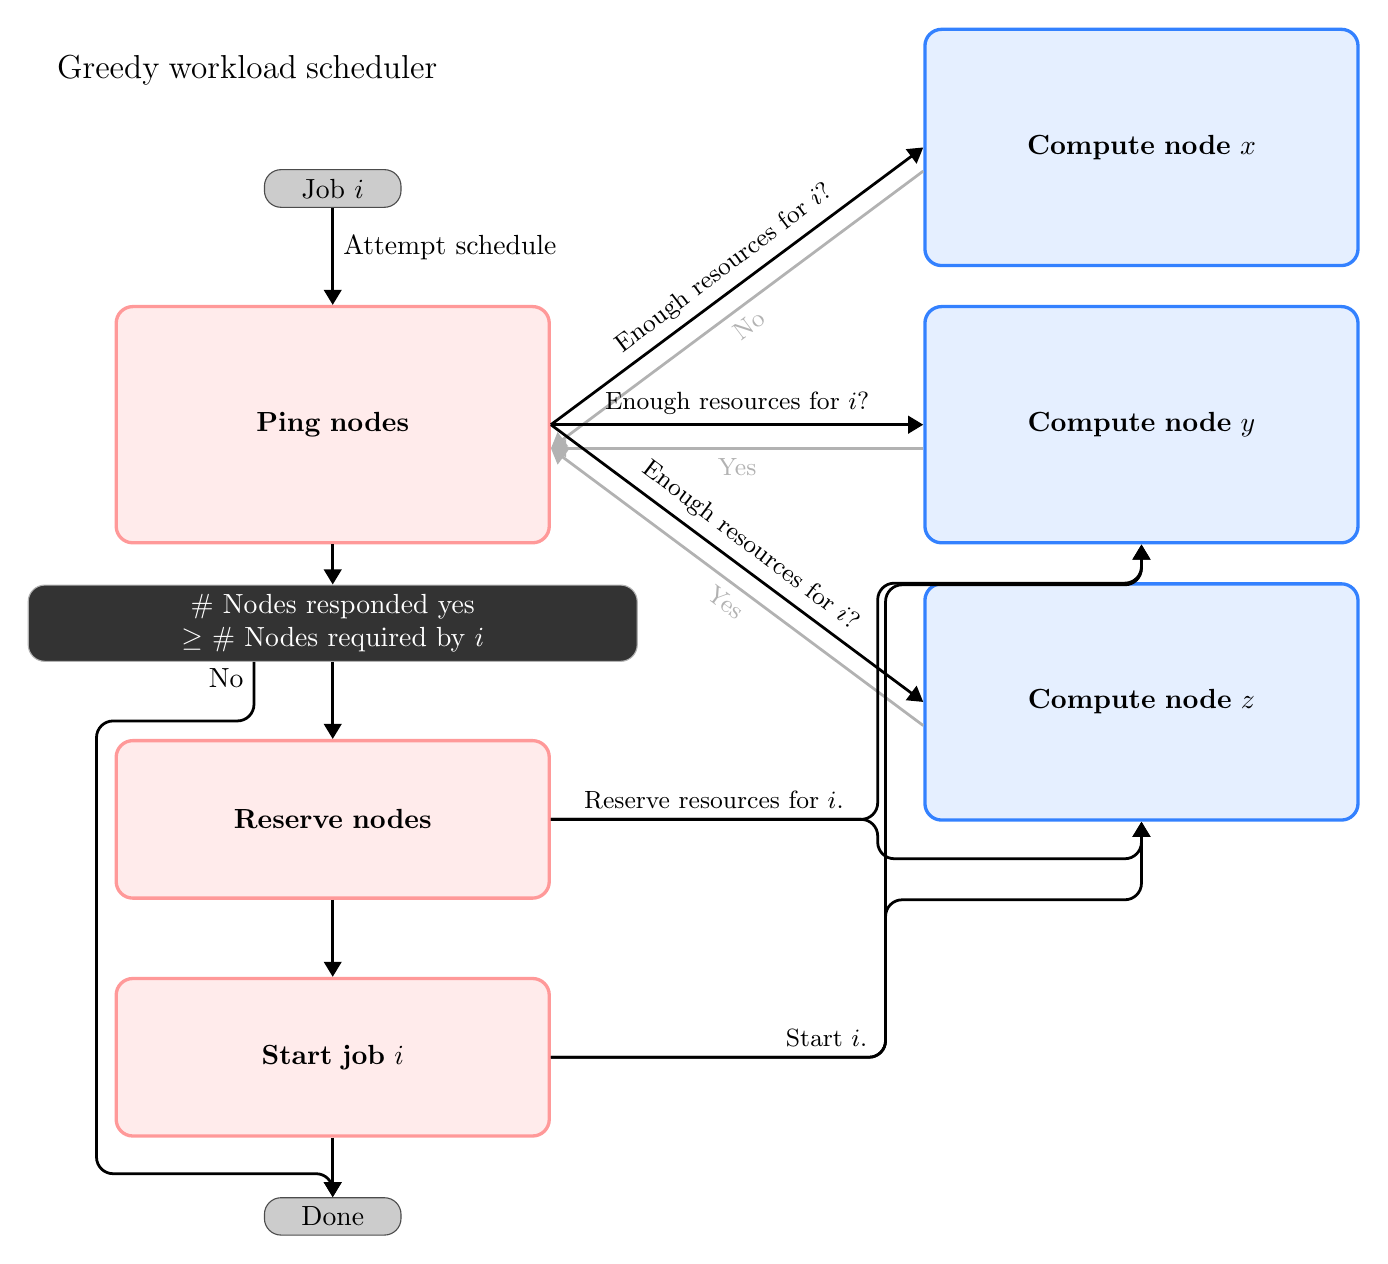
\begin{tikzpicture}[rounded corners=6, align=left]
    \begin{scope}[local bounding box=model]
        \node[\drawcolor, solid, text width=70mm, minimum width=75mm] at (0, 0) (title) {\large Greedy workload scheduler};

        \node[whitemodule] at ($(title) + (0, -1.5)$) (incomingJob) {Job $i$};

        \node[redmodule] at ($(incomingJob) + (0, -3)$) (headScheduler) {\textbf{Ping nodes}};

        \node[bluemodule] at ($(headScheduler.east) + (7.5, 0.0)$) (computeSchedulerB) {\textbf{Compute node $y$}};

        \node[bluemodule] at ($(computeSchedulerB.north) + (0.0, +2.0)$) (computeSchedulerA) {\textbf{Compute node $x$}};

        \node[bluemodule] at ($(computeSchedulerB.south) + (0.0, -2.0)$) (computeSchedulerC) {\textbf{Compute node $z$}};

        \node[darkmodule] at ($(headScheduler.south) + (0, -1.0)$) (condition) {\# Nodes responded yes $\geq$ \# Nodes required by $i$};

        \node[redmodule, minimum height=20mm] at ($(condition.south) + (0, -2)$) (reserveNodes) {\textbf{Reserve nodes}};

        \node[redmodule, minimum height=20mm] at ($(reserveNodes.south) + (0, -2)$) (startJob) {\textbf{Start job $i$}};

        \node[whitemodule] at ($(startJob.south) + (0, -1)$) (done) {Done};

        % Arrows
        \draw[\drawcolor, -{Triangle}, line width=1pt] (incomingJob.south) node [right, yshift=-5mm] {Attempt schedule} to (headScheduler.north);
        \draw[faded, -{Triangle}, line width=1pt] ($(computeSchedulerA.west) + (0, -3mm)$) -- ($(headScheduler.east) + (0, -3mm)$) node [below, midway, rotate=37] {\small No};
        \draw[faded, -{Triangle}, line width=1pt] ($(computeSchedulerB.west) + (0, -3mm)$) -- ($(headScheduler.east) + (0, -3mm)$) node [below, midway, rotate=0] {\small Yes};
        \draw[faded, -{Triangle}, line width=1pt] ($(computeSchedulerC.west) + (0, -3mm)$) -- ($(headScheduler.east) + (0, -3mm)$) node [below, midway, rotate=-37] {\small Yes};
        \draw[\drawcolor, -{Triangle}, line width=1pt] (headScheduler.east) -- (computeSchedulerA.west) node [above, midway, rotate=37] {\small Enough resources for $i$?};
        \draw[\drawcolor, -{Triangle}, line width=1pt] (headScheduler.east) -- (computeSchedulerB.west) node [above, midway] {\small Enough resources for $i$?};
        \draw[\drawcolor, -{Triangle}, line width=1pt] (headScheduler.east) -- (computeSchedulerC.west) node [above, midway, rotate=-37] {\small Enough resources for $i$?};

        \draw[\drawcolor, -{Triangle}, line width=1pt] (headScheduler.south) -- (condition.north) node [midway, right] {};

        \draw[\drawcolor, -{Triangle}, line width=1pt] ($(condition.south) + (-1.0, 0.0)$) node [left, yshift=-2.0mm] {No} to 
            ($(condition.south) + (-1.0, -0.75)$) to 
            ($(condition.south) + (-3.0, -0.75)$) to 
            ($(condition.south) + (-3.0, -6.5)$) to 
            ($(condition.south) + (+0.0, -6.5)$) to 
            (done.north);

        \draw[\drawcolor, -{Triangle}, line width=1pt] (condition.south) -- (reserveNodes.north) node [midway, right] {};

        \draw[\drawcolor, -{Triangle}, line width=1pt] (reserveNodes.east) to 
            ($(reserveNodes.east) + (2.07, +0.0)$) node [above] {\small Reserve resources for $i$.} to
            ($(reserveNodes.east) + (4.15, +0.0)$) to
            ($(reserveNodes.east) + (4.15, -0.5)$) to
            ($(reserveNodes.east) + (7.50, -0.5)$) to
            (computeSchedulerC.south);
        \draw[\drawcolor, -{Triangle}, line width=1pt] (reserveNodes.east) to 
            ($(reserveNodes.east) + (4.15, +0.0)$) to
            ($(reserveNodes.east) + (4.15, +3.0)$) to
            ($(reserveNodes.east) + (7.50, +3.0)$) to
            (computeSchedulerB.south);

        \draw[\drawcolor, -{Triangle}, line width=1pt] (reserveNodes.south) -- (startJob.north) node [midway, right] {};

        \draw[\drawcolor, -{Triangle}, line width=1pt] (startJob.east) to 
            ($(startJob.east) + (3.50, 0.0)$) node [above] {\small Start $i$.} to
            ($(startJob.east) + (4.25, 0.0)$) to
            ($(startJob.east) + (4.25, 2.0)$) to
            ($(startJob.east) + (7.50, 2.0)$) to
            (computeSchedulerC.south);
        \draw[\drawcolor, -{Triangle}, line width=1pt] (startJob.east) to 
            ($(startJob.east) + (3.50, 0.0)$) to
            ($(startJob.east) + (4.25, 0.0)$) to
            ($(startJob.east) + (4.25, 6.0)$) to
            ($(startJob.east) + (7.50, 6.0)$) to
            (computeSchedulerB.south);

        \draw[\drawcolor, -{Triangle}, line width=1pt] (startJob.south) -- (done.north) node [midway, right] {};

    \end{scope}

\end{tikzpicture}
\end{document}
